\chapter{Delvers}

\section{Delvers of Orth}
The champions of this story are the delvers also known as cave raiders. Their mission is to explore the abyss, retrieve its many riches, and discover its many mysteries. However, their descent is fraught with danger and unforeseen encounters, often to their untimely demise. They are considered folk heroes by the \textit{town of Orth}. The town is built around the edge of the abyss. 

\section{Background \& Motives}

Delver's motivations for delving the abyss are varied. Some are drawn to it from a competitive aspect, others for its many wonderous treasures, and others from pure curiosity about its many secrets. What they all have in common is their undying desire to brave the abyss to attain their goal.

\begin{quotebox}
"If it was between dying of old age, or of some stupid thing like a heart attack... I'd want to die exploring the great unknown, and satisfying that urge to see the endless nameless." \newline\textit{Øbserver, a blue whistle}
\end{quotebox}

\header{Whistle Illustrations}

\begin{center}
\begin{tabular}{c}
\adjustbox{trim=0 0 0 0,clip}{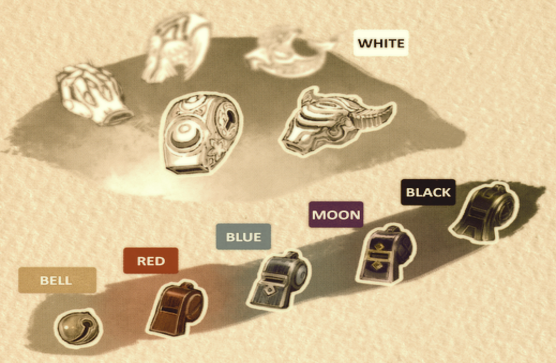
\includegraphics[width=7.5cm]{img/delvers/1.png}} \\
 \end{tabular}
\captionof{figure}{e) Descending into the 6th layer is known as the Last Dive. Curses beyond this point are severe and lethal for humans.}
\end{center}

\section{Delvers' Whistles}
All delvers (*) are equipped with a whistle. They represents their wearers social status within Orth and their expertise as delvers of the Abyss. Experienced delvers can travel further down without severe consequences. They have a better understanding of the layout and dangers of each of the layers. 

In terms of mechanics delvers' rank describe which layers is most appropriate for their level. See table 1.1.

\header{Delvers' Rank}
\begin{dndtable}[llX]
    \textbf{Title} & \textbf{Position} & \textbf{Deepest Layer}\\
    Bell whistle & Student & Surface \\
    Red whistle & Apprentice & 1st \\
    Blue whistle & Adept & 2rd \\
    Moon whistle & Teacher & 3rd \\
    Black whistle & Expert & 4th \\
    White whistle & Legendary & 5th+\footnote{See section "The Last Dive"\ref{se:thelastdive}, p. \pageref{se:thelastdive}}  \\
\end{dndtable}
\label{tab:colors}

\subsection{Bell Whistles}
Work in Progress.

\subsection{Red Whistles}
The apprentices. Red Whistles are rookie delvers who have a decent knowledge of the abyss and have descended up to the first layer on their own. It is a common rank for prepubescent kids who have studied since an early age. One obtains a red whistle and the official title of delver after they first descent to the abyss. While they're fairly knowledgeable, red whistles lack the physical fortitude to get very deep, so they're only allowed to descend up to 550 meters. Going any deeper would be treated as an accident or a rebellious behavior, and a rescue party would be sent to retrieve them. If a red whistle somehow managed to descend 1350 meters, it is treated as suicide and search parties are called off. 

\subsection{Blue Whistles}
The adepts. Blue Whistles are more experienced delvers who managed to proved themselves. They're allowed to delve up to the second layer of the abyss, so they most likely possess an acceptable fighting ability to fend off from the beasts of the forest of temptation. Typically and with the appropriate training, one attains the rank of blue whistle at the age of 15, though there are exceptions to this. 

\subsection{Moon Whistles}
The teachers. Moon Whistles are highly proficient delvers that carry an extensive knowledge of the abyss. They can delve up to the third layer safely, so their delving ability is in a completely different level to Blue Whistles. They're considered experienced enough to serve as teachers for the newer generations. 

\subsection{Black Whistles}
The experts. Black Whistles are extremely talented delvers that have mastered the delving techniques of delvers. They can reach up to the fourth layer of the abyss, which is the point in which the strains of ascension can really make one touch insanity. Black Whistles also sometimes work under white whistles as subordinates, and assist them in their expeditions. 

\subsection{White Whistles}
The legends. White Whistles are considered to be the greatest delvers of all. Their achievements have changed the world and their discoveries astonished all, turning into spectacular historical figures. They're named after their unique persona and reach a whole new level incomparable to that of other delvers. They're armed to the teeth with artifacts of the abyss, and represent a formidable force. Because of their status, any information that is officially passed by them is considered a fact, no matter how absurd.

Only a handful of delvers attain this legendary rank, and only five white whistles are known:

\header{Known White Whistles}
\begin{dndtable}[lX]
  \textbf{Name} & \textbf{Title} \\
  Lyza the Annihilator & The Lord of Annihilation \\
  Ozen the Immovable & The Immovable Sovereign \\
  Bondrewd the Novel & The Lord of Dawn \\
  Srajo the Obscure & The Lord of Mystery \\
  Wakuna & The Lord of Guidance \\
\end{dndtable}

\subsubsection{The Last Dive} \label{se:thelastdive}
White Whistle don't have any depth limit, however since the strains of ascension make it humanly impossible to survive the ascent from the 6th layer, for most of their life the 5th layer is their limit. At some point when they make the decision, a white whistle will descend to the inviolable 6th layer. Since return from this point is impossible, this descent is called the "Last Dive" and it represents the most important point of their career, delving into largely unknown territory.

\section{Equipment}
Work in Progress.